
\documentclass{article}
\usepackage[utf8]{inputenc}
\usepackage[spanish]{babel}
\usepackage{graphicx}
\usepackage{geometry}
\usepackage{enumerate}
\usepackage{titlesec}
\usepackage{float}

\geometry{letterpaper, margin = 1.5cm}

%Datos de la Portada
\title{Introduccion a la Programacion \\ Practica 2}
\author{Medina Martinez Jonathan Jason \\ 2023640061}
\date{06 de marzo de 2023}

\begin{document} %Inicio del Documento

\fontsize{12}{16}\selectfont

\begin{figure}[t] %Logos Portada


\includegraphics[width=2.5 cm]{Logo1.jpeg}
\hfill

\includegraphics[width=3 cm]{Logo2.png}

\end{figure}

\maketitle %Titulo Portada
\newpage

\tableofcontents %Indice
\newpage

\section{Objetivo}

Practicar el uso de variables, constantes y operadores.

\
\
\

\section{Introducción}

En esta practica se realizaran diversos programas en c utilizando diversos operadores, variables y constantes.

\newpage

\section{Desarrollo}
\subsection{Programa 1}

Programa que calcule el area y el perımetro de un cırculo. El programa debera solicitar al usuario el valor del radio y debera mostrar el area y el perımetro calculado. Debera definir $\pi$ como constante.

\

\begin{figure}[H]
    \centering
    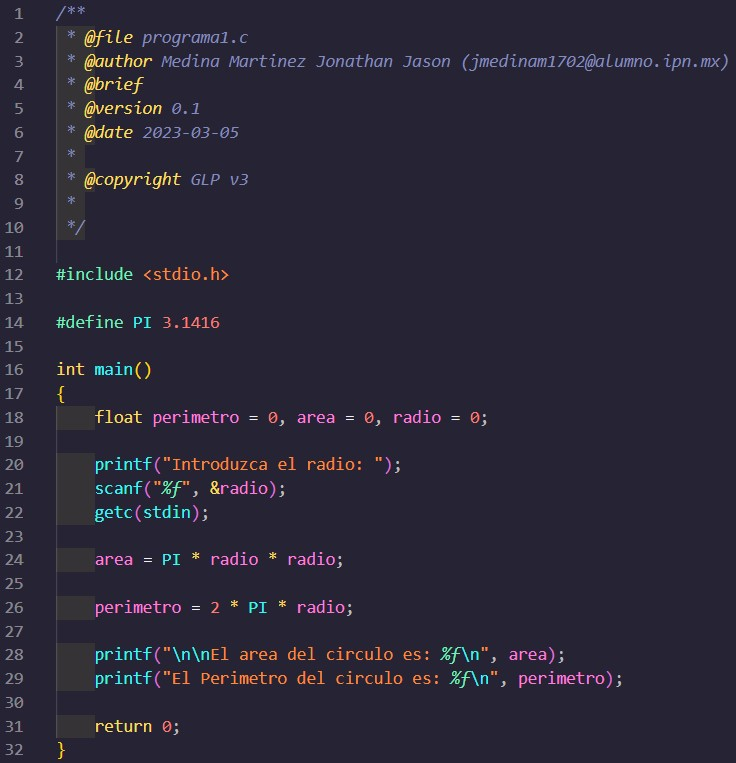
\includegraphics[height = 19cm]{img1.jpg}
\end{figure}

\subsection{Programa 2}

Programa que permita al usuario obtener la raız enesima de un numero entero positivo mayor a 0. Para esto, debera hacerlo con logaritmos.

\begin{figure}[H]
    \centering
    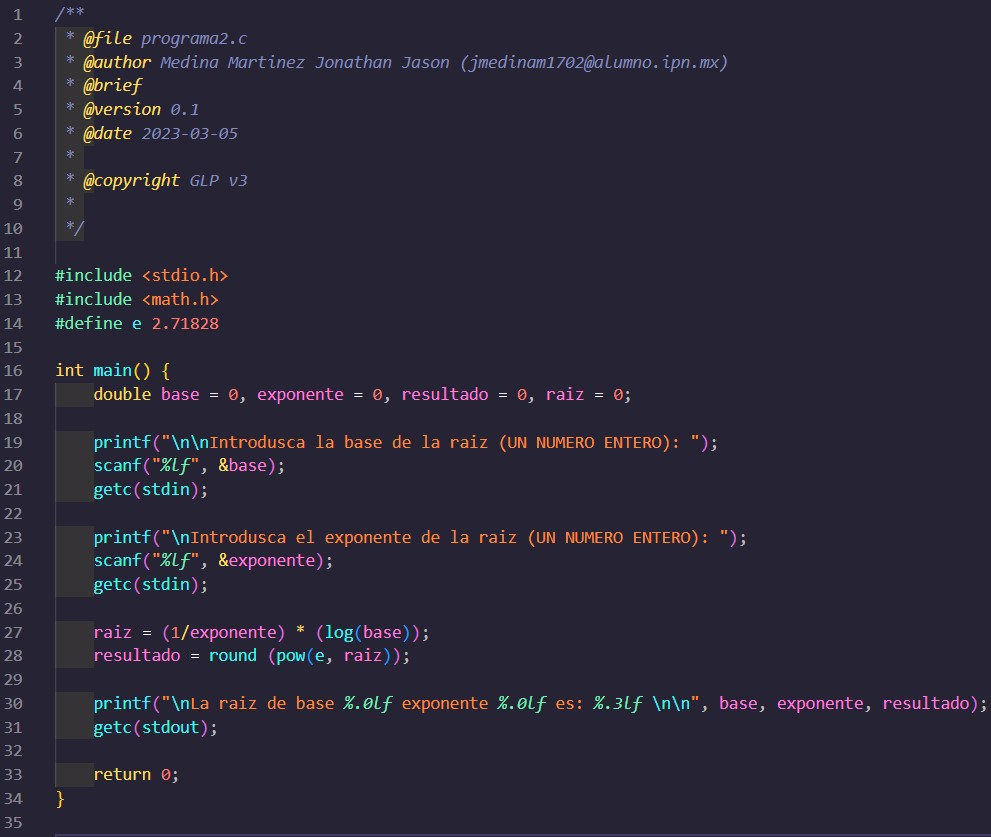
\includegraphics[width = 12cm]{img2.jpg}
    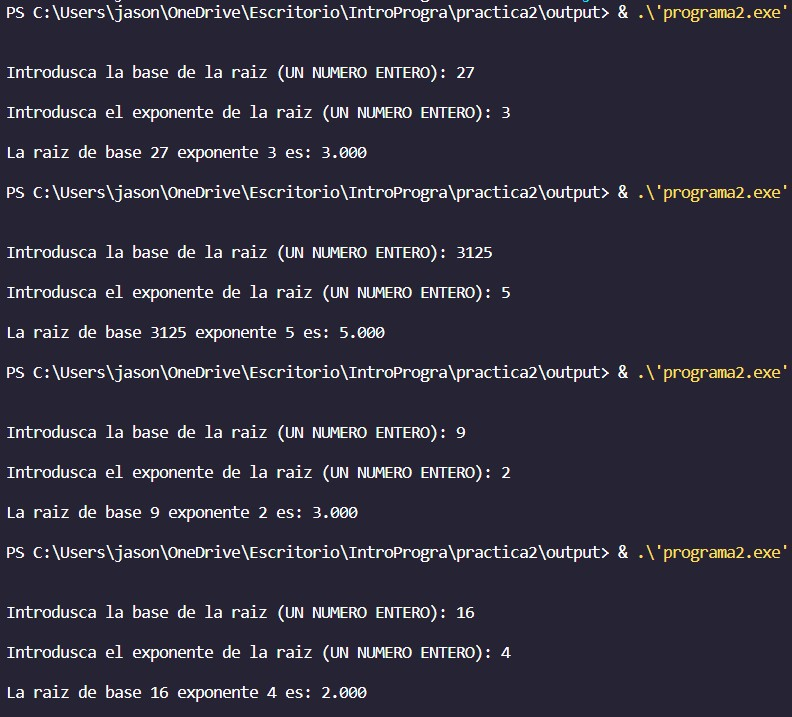
\includegraphics[width = 12cm]{img2a.jpg}
\end{figure}

\subsection{Programa 3}

Programa que calcule la distancia entre dos puntos proporcionados por el usuario. Recuerde, dados los puntos $A(x1, y1)$ y $B(x2, y2)$, la distancia se define como

$$d(A, B) = \sqrt{(x_2 - x_1)^2 + (y_2 - y_1)^2}$$

\begin{figure}[H]
    \centering
    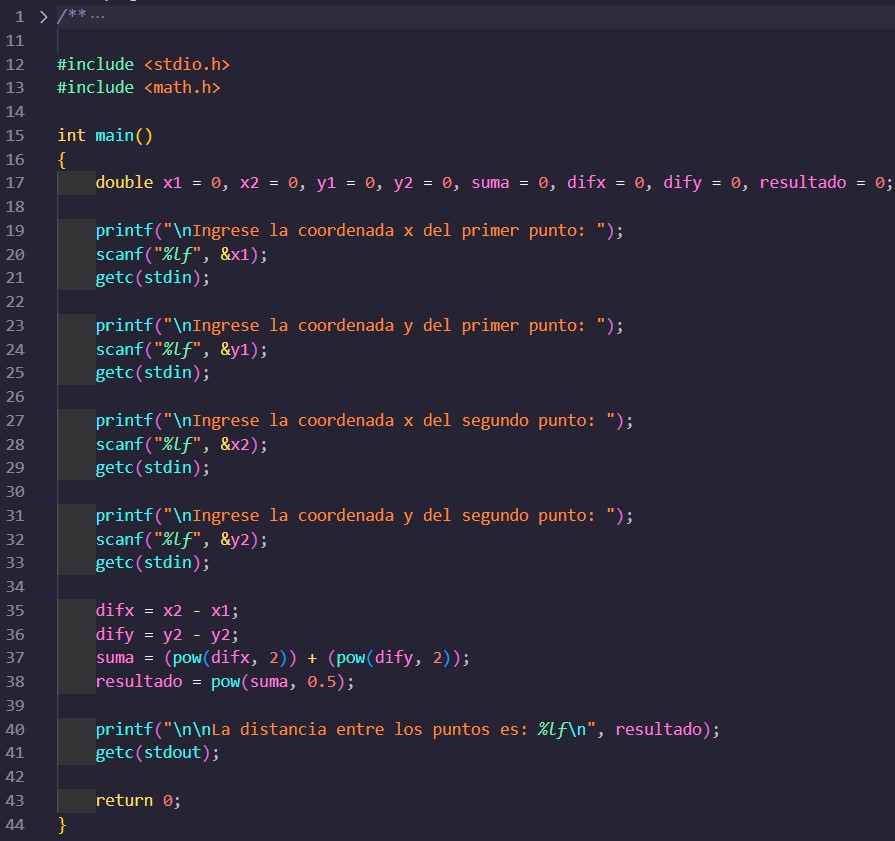
\includegraphics[height = 17cm]{img3.jpg}
\end{figure}

\newpage

\subsection{Programa 4}

Programa que solicite al usuario un numero y le indique si es par o impar. Debera utilizar el operador modulo, el operador AND y el operador ternario ? :

\begin{figure}[H]
    \centering
    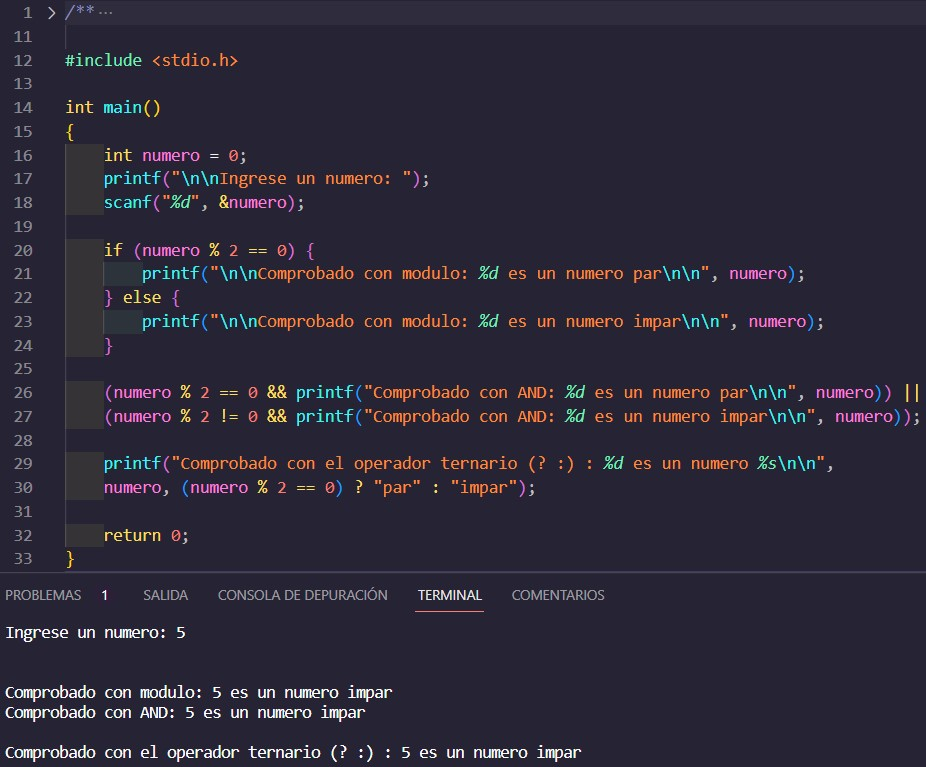
\includegraphics[height = 15.5cm]{img4.jpg}
\end{figure}

\newpage

\subsection{Programa 5}

Programa que permita convertir de grados Centıgrados a grados Fahrenheit.

\begin{figure}[H]
    \centering
    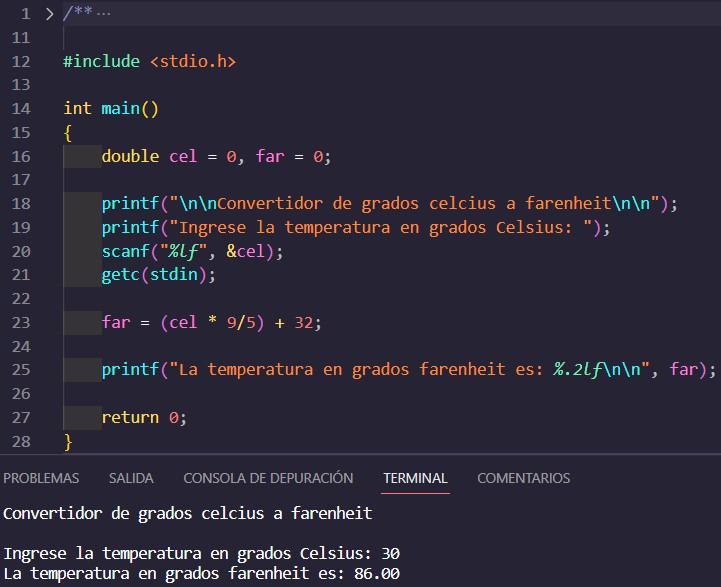
\includegraphics[height = 15cm]{img5.jpg}
\end{figure}

\newpage

\subsection{Programa 6}

Programa que permita convertir de grados Fahrenheit a grados Centıgrados.

\begin{figure}[H]
    \centering
    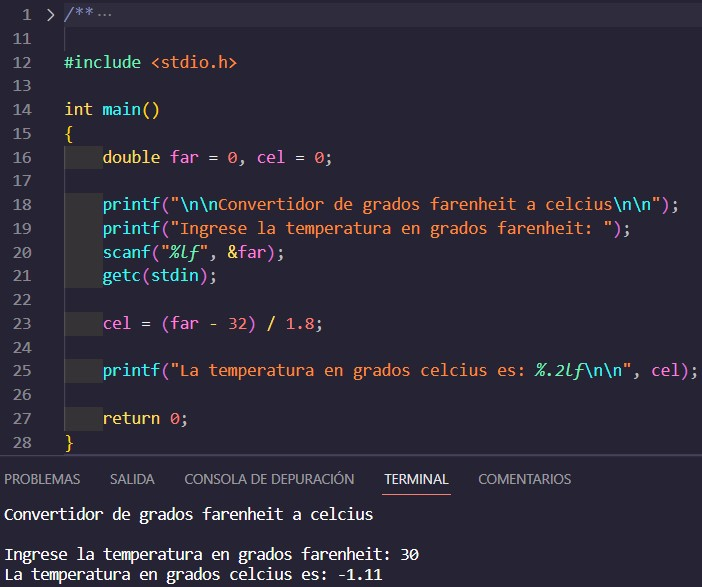
\includegraphics[height = 15cm]{img6.jpg}
\end{figure}

\newpage

\subsection{Programa 7}

Programa que permita calcular el enesimo numero de la sucesion de Fibonacci sin la necesidad de producir todos los numeros anteriores.

\begin{figure}[H]
    \centering
    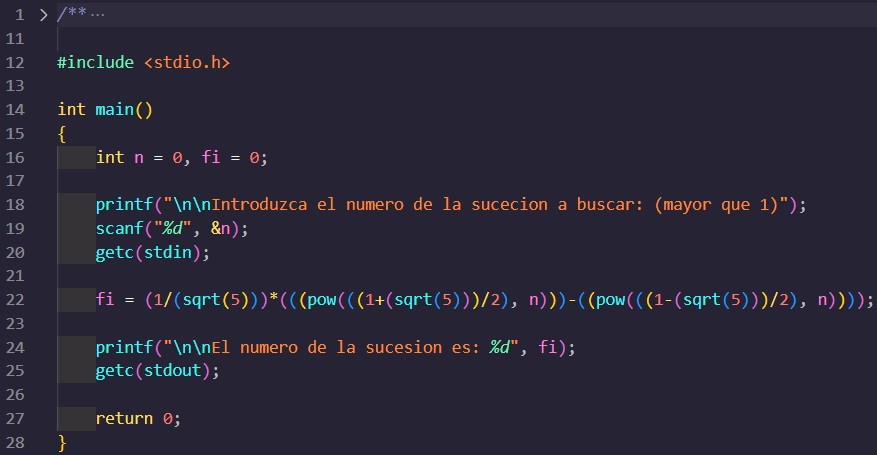
\includegraphics[height = 9.5cm]{img7.jpg}
\end{figure}

\
\
\
\

\section{Conclusion}

En esta practica realizamos distintos tipos de operaciones y funciones en c a travez de diversos operadores, constantes y variables.

\end{document}